\section{Benchmark Dataset Curation}
\label{sec:data_curation}

\begin{figure*}[t!]
\begin{center}
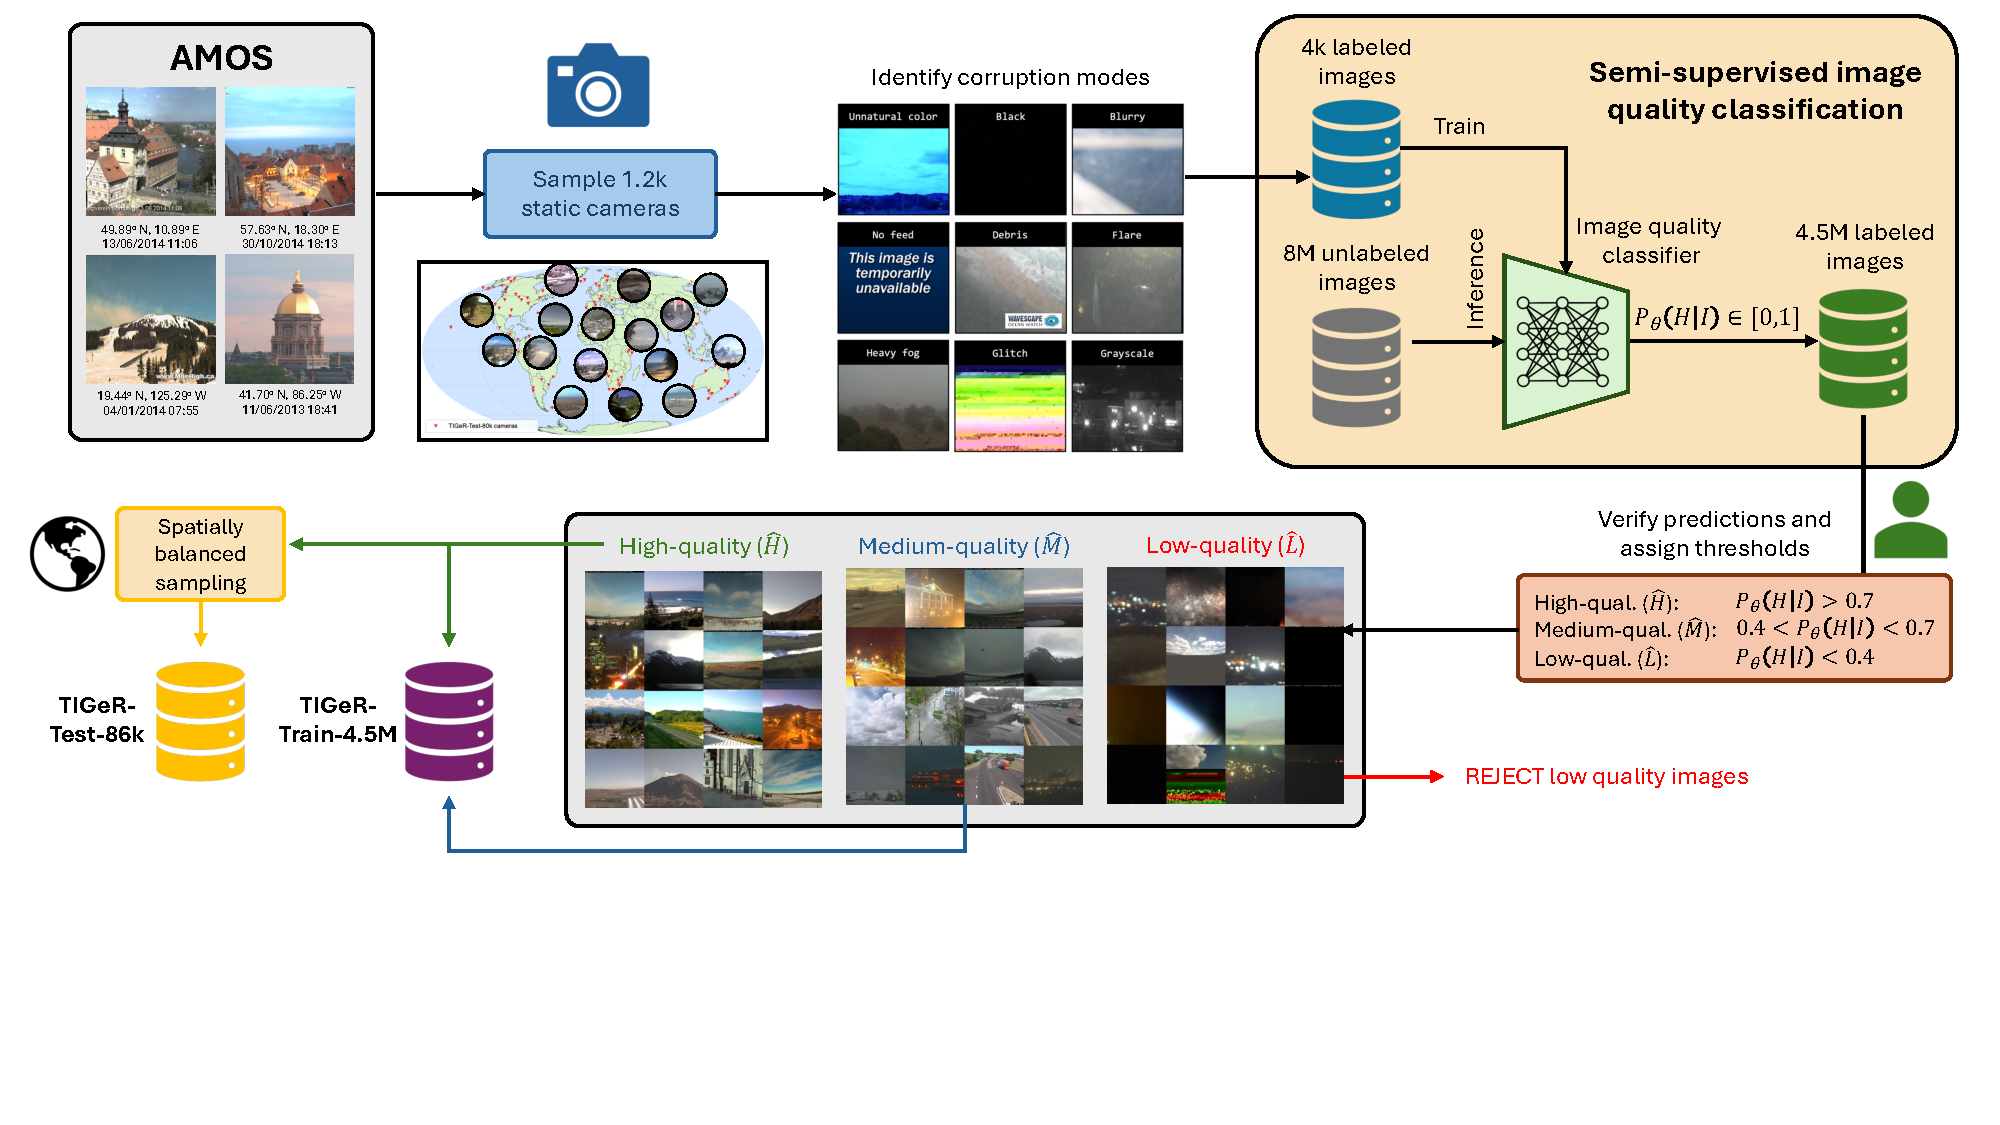
\includegraphics[width=0.95\textwidth]{figures/data_pipeline_camera_ready.pdf}
\end{center}
\vspace{-1em}
\caption{
\textbf{Benchmark dataset curation pipeline.} Starting from the AMOS corpus, we randomly sample 1,255 static cameras with broad global coverage and identify diverse corruption modes. We manually label 4,000 images for quality, train a semi-supervised image quality classifier on frozen visual features, and apply it to 8M unlabeled frames to predict a quality score $P(H|I)$. Using thresholds $T_H{=}0.7$ and $T_L{=}0.4$, images are partitioned into high-, medium-, and low-quality subsets, and low-quality frames are discarded. High-quality images are then used to construct a geographically balanced test set by sampling cameras across $10^\circ \times 10^\circ$ latitude-longitude bins and retaining only cameras with at least 500 frames spanning a year, while the remaining high- and medium-quality images form the training set. The resulting benchmark contains 4.5M training images and 86k test images, with no camera overlap between splits.
}
\label{fig:data_pipeline}
\end{figure*}

Constructing a dataset suitable for time-aware geolocalization presents significant challenges. One potential dataset is AMOS \cite{jacobs07amos, jacobs09webcamgis}, which  provides a vast collection of static outdoor imagery distributed across diverse regions, months, and times-of-day, however, its raw form is highly unsuitable for direct use. The dataset suffers from pervasive noise and corruption, stemming from both hardware limitations and environmental conditions. Many cameras frequently generate unusable frames due to broken hardware or missing camera feeds. Low-cost sensors introduce additive Gaussian-like noise and compression artifacts, while night time images often collapse into near-black frames with severely limited dynamic range. Other failure modes include misconfigured sensors producing banding or dead pixels, placeholders or stale frames with uniform content, and weather-induced distortions (rain, snow, fog) that obscure critical scene details. Without careful filtering, these corruptions overwhelm useful signal, making curation a central challenge. We list all the corruption modes and describe them in detail in the supplementary section~\ref{sup:sec_corruption}.

To overcome these challenges, we design a multi-stage curation pipeline (Figure~\ref{fig:data_pipeline}), that systematically filters noise while preserving both geographic and temporal diversity. To ensure global coverage, we begin by randomly sampling 1,255 cameras from the AMOS dataset across both hemispheres and multiple continents. To build a supervised filtering model, we manually annotate 4,000 samples into high- and low-quality categories, capturing the diverse corruption modes described above. Formally, if an image $I$ has any form of corruption, we assign it to the low-quality set $L$ with a label $q=0$; otherwise it is placed in the high-quality set $H$ with $q=1$. 

Using these seed sets, we train a lightweight classifier on frozen CLIP \cite{clip} and DINOv2 \cite{oquab2023dinov2} visual features, with a linear probe optimized for binary quality prediction. The output of the model is a confidence score $p(q=H|I) \in [0,1]$, indicating the probability that an image is of high-quality. We then evaluate the model's performance on a hold-out set of 400 images resulting in a binary classification accuracy of 91\%. Based on the cumulative score distribution to select two thresholds $T_H=0.7$ and $T_L=0.4$ which we use to group the predictions into high- ($\hat H$), medium- ($\hat M$), and low-quality ($\hat L$) sets as follows:
\begin{equation}
    I \in \begin{cases}
        \hat H, & \mathrm{if} \quad P(H|I) \geq T_H \\
        \hat M, & \mathrm{if} \quad T_L \leq P(H|I) < T_H  \\
        \hat L, & \mathrm{if} \quad P(H|I) < T_L
    \end{cases}.
\end{equation}

The images assigned to the low-quality set $\hat L$ are removed from the dataset, since excessive noise can obscure the geo-temporal signals needed to train and evaluate our model. In contrast, the high-quality images in $\hat H$ are well suited for building the test set, as they typically exhibit good illumination, mild weather conditions, and reliable camera feeds. To construct a representative benchmark, we seek a test set with a balanced geographic distribution across both hemispheres. This is particularly important for tasks involving time-of-year, since seasonal appearance is strongly correlated with calendar month, while seasons are inverted between the Northern and Southern Hemispheres.

Beyond balancing the number of test images across hemispheres, we also aim to avoid over-representing regions with denser camera coverage. To this end, we partition the globe into $10^\circ \times 10^\circ$ latitude-longitude bins and select cameras that are approximately evenly distributed across them. From these candidate cameras, we retain only those with at least 500 frames spanning a full year, ensuring coverage across multiple months and hours at each location. All remaining cameras from the high- and medium-quality subsets are assigned to the training set. Importantly, the training and test splits share no cameras, allowing our evaluation to better measure the model’s ability to generalize to unseen locations.

\begin{figure}[t]
\begin{center}
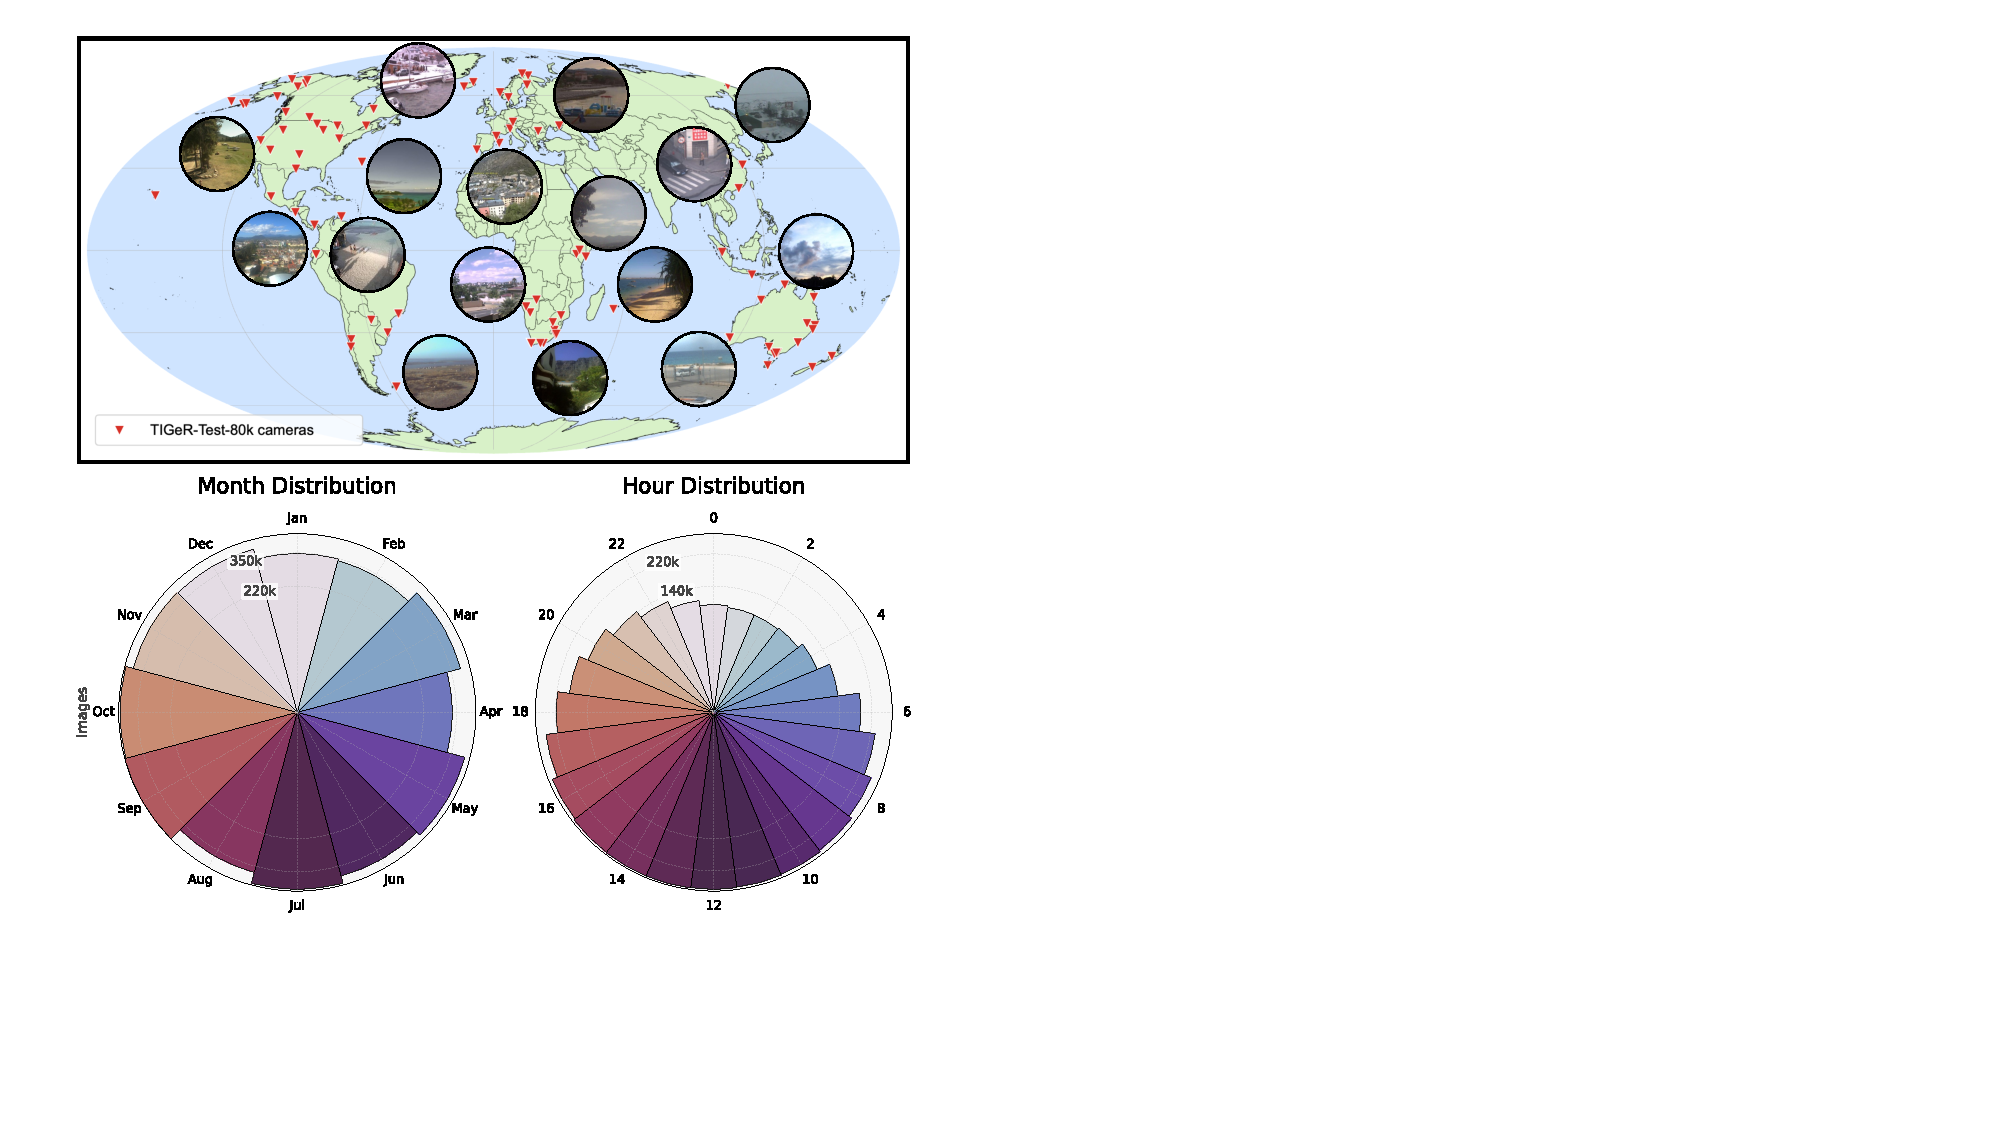
\includegraphics[width=0.9\linewidth]{figures/test_dustribution_cam_ready.pdf}
\end{center}
\vspace{-1em}
\caption{\textbf{Dataset statistics and distributions.}
\textbf{Top}: Geographical distribution of camera locations across the world in the proposed dataset, showing wide coverage across multiple continents.
\textbf{Left}: Time-of-year (month) distribution of the captured images.
\textbf{Right}: Time-of-day (hour) distribution of the captured images.
}
\label{fig:dataset_dist}
\end{figure}

After all the filtering stages, the curated dataset contains $4.5M$ training images and $86k$ test images. Figure~\ref{fig:dataset_dist} illustrates the resulting geographic and temporal distributions. This pipeline transforms the noisy AMOS corpus into a clean, balanced, and diverse benchmark, enabling robust training and reliable evaluation for downstream geo-localization and time prediction tasks.
